% $ platex body
% $ dvipdfmx body

\documentclass[a4j]{jarticle}

\title{「西洋音楽の歴史と理論」報告課題}
\author{KR17074 山内 拓弥}
\date{平成29年9月xx日}
\usepackage{colortbl}
\usepackage[dvipdfmx]{graphicx}
%\renewcommand{\thesection}{課題\arabic{section}}
%\renewcommand{\thesubsection}{}

\begin{document}

%\maketitle

\section{中世封建社会の解体}

ヨーロッパ中世の封建社会において、
国王である主君から荘園と呼ばれる領土を与えられた領主は、
その領土の見返りとして軍事的に奉仕する契約を結ぶ。
主君が契約を破れば、臣下である領主も契約を拒否する権利があった。
また、領主は契約の内容以上に主君に尽くす義務は無かった。
このように、中世ヨーロッパの封建制は、
領主の立場が比較的強かった。
この時期、ヨーロッパで最も権力を持っていたのは、ローマ教皇であった。
しかし、1096年から1291年にわたる十字軍の遠征とその失敗により、
ローマ教皇の権威が低下した。
また、十字軍の遠征により、領主が疲弊、没落し、
国王が領主の土地を没収し、国王の権力が高まった。
14世紀頃から貨幣経済がヨーロッパにいきわたり、
余剰生産物の売却などにより農民の地位が向上した。
また、このような社会の変化に対応できずに没落した領主の土地を大商人が購入し、
新しい領主となっていった。
荘園制を基盤とする封建社会は次第に解体し、
貨幣経済と王権を基盤とする社会に変わっていく。

\section{ルネサンス時代}

オスマン帝国

大航海時代
羅針盤
活版印刷
火薬

1488
バルトロメウ=ディアス
喜望峰

1498
ヴァスコ=ダ=ガマ
インド航路

1492
コロンブス
アメリカ大陸
アメリゴ=ヴェスプッチ

1500
カブラル
ブラジル

1522
マゼラン一行
世界一周

1521
コルテス
アステカ王国を征服

1533
ピサロ
インカ帝国を滅ぼす

アメリカから銀がヨーロッパに流入。
西ヨーロッパでインフレ

ダンテ 神曲
ラテン語ではなく、イタリアのトスカーナ地方の口語。

ボッティチェッリ
ヴィーナスの誕生 ギリシャ神話 キリスト教にとっては異教
レオナルド=ダ=ビンチ、ラファエロ

フィレンチェの大商人メディチ家、ローマ教皇がルネサンスを支援。

マキャヴェリ
道徳や宗教とは切り離した現実的な政治学
君主は場合によっては権謀術数も必要である。

コペルニクス
地動説

グーテンベルク
活版印刷を発明

聖ピエトロ大聖堂の大改修
贖宥状
1517 95ヶ条の論題
1521 教会から破門
プロテスタント
ルターの主張は、活版印刷によりドイツ国内に広がった。
救済は信仰によってのみもたらされる
聖書が唯一の拠り所である
神の前に万人は平等であり、信徒は全て伝道者である

カトリックのミサ典礼
聖歌は修道士や聖歌隊によって歌われる
ルター
礼拝に参列した会衆が共に歌って神を賛美し祈りを捧げる
ドイツ語の式文、コラールを定める

カルヴァン
現世での勤労と禁欲が救いをもたらす
魂の救済は神によって既に決定されており、
人間の努力では変更不可能
予定説
人々はとにかく日々の労働を勤勉に行うしかない。
当時の西ヨーロッパの新興階層である商工業者が支持

イギリス
ヘンリー8世
王妃との離婚を認めない教皇に反発
カトリックとプロテスタントの折衷
熱心なプロテスタントの信者をピューリタンという

カトリック
対抗宗教改革
1545
トリエント公会議 1545-1563
卑猥で不純な音楽を排除すること
などが決議
複雑なポリフォニーに非難


\begin{table}[tb]
 \begin{center}
  \caption{西ヨーロッパ中世とルネサンスの比較}
  \label{tab:comparison}
  \begin{tabular}{|l|l|} \hline
  中世                       & ルネサンス                         \\
  \hline \hline
  教皇が絶大な権力を持つ。   & 教皇の権威が低下、国王が力を持つ。 \\ \hline
  神が中心。                 & 人間が中心。                       \\ \hline
  非写実的な絵画、彫刻。     & 写実的な絵画、彫刻。遠近法。       \\ \hline
  教会による人体解剖の禁止。 & 人体解剖図が描かれる。             \\ \hline
  地球は平坦、天動説。       & 地球は球形、地動説。               \\ \hline
  和音は、神学的理論を優先。 & 和音は、人間の聴覚を優先。         \\
  5度音程が中心。            & 3度、6度のやわらかい響きを多用。   \\ \hline
  \end{tabular}
 \end{center}
\end{table}

\section{ルネサンスの音楽}

\begin{figure}[tb]
 \begin{center}
  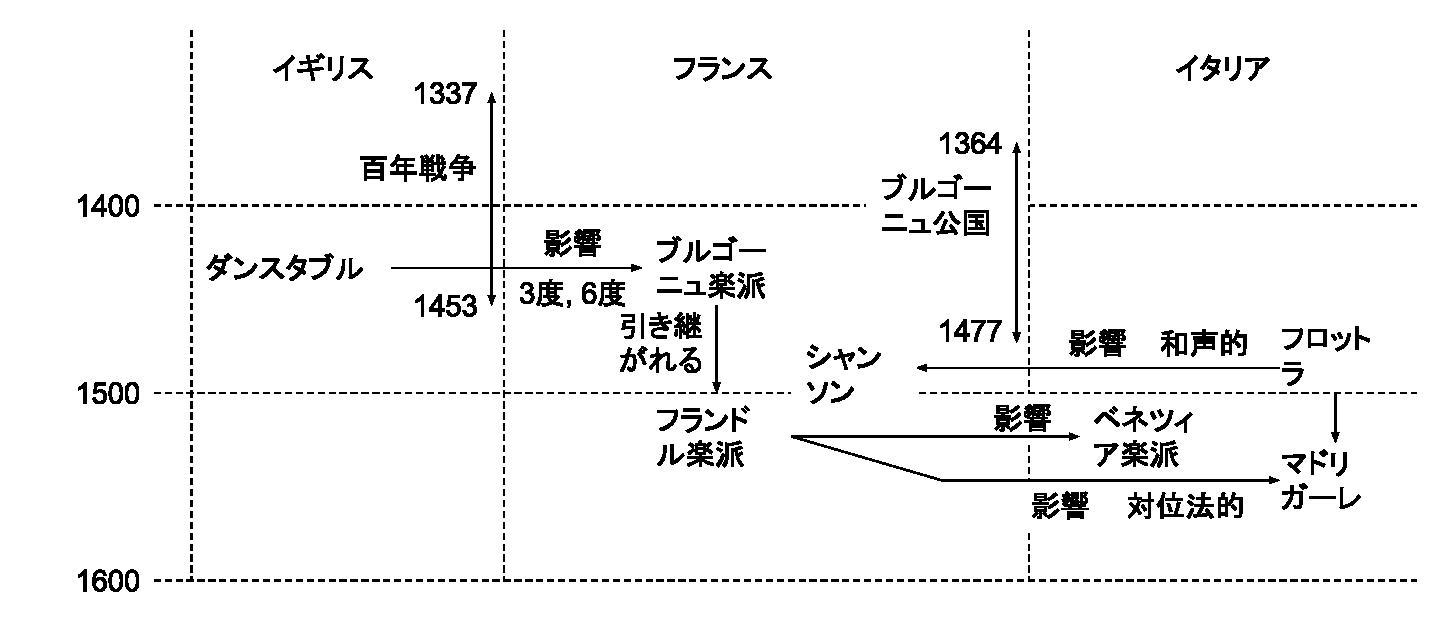
\includegraphics[width=\hsize]{fig/renaissance_summary.eps}
  \caption{ルネサンス音楽概略}
  \label{fig:renaissance_summary}
 \end{center}
\end{figure}

\end{document}
